\chapter{Metodologi dan Desain Sistem}
\section{Metodologi Penelitian}
Metodologi yang digunakan menyelesaikan tugas akhir, ditunjukkan pada gambar diaram alir \ref{flow:fig_flow_method}. Berikut penjelasan tiap tahap pada diagram alir:
\begin{enumerate}
	\item \textbf{Studi literatur} \\
	Pada tahap ini penulis mengumpulkan literatur seperti buku, artikel dan \textit{paper} yang berguna menjadi landasan informasi pada penelitian. Hasil tahap ini ialah fakta dan teori serta masalah yang dihadapi.
	\item \textbf{Perancangan Sistem} \\
	Pada tahap ini penulis memilah masalah yang dapat diselesaikan berdasarkan fakta dan teori yang telah dikumpulkan. Hasil tahap ini ialah rancangan sistem yang diajukan sebagai solusi.
	\item \textbf{Persiapan Data Uji} \\
	Pada tahap ini penulis mempersiapkan data yang telah tervalidasi kebenarannya untuk dijadikan input pengujian. Hasil tahap ini ialah dataset yang telah dianotasi.
	\item \textbf{Implementasi} \\
	Pada tahap ini penulis menerapkan rancangan sistem baik yang berupa \textit{software} maupun \textit{hardware}. Hasil tahap ini ialah \textit{software} dan \textit{hardware} yang dapat berjalan tanpa masalah.
	\item \textbf{Pengujian dan Analisis} \\
	Pada tahap ini penulis melakukan pengujian terhadap sistem yang dibangun menggunakan data uji dan parameter pengujian. Jika ditemukan ada masalah teknis ataupun kemungkinan melakukan peningkatan performansi maka penulis akan kembali ke tahap implementasi. Hasil tahap ini ialah \textit{software} dan \textit{hardware} dengan konfigurasi terbaik yang ditemukan.
	\item \textbf{Penyusunan Laporan} \\
	Pada tahap ini penulis melakukan penulisan laporan hasil akhir dari tugas akhir. Hasil dari tahap ini berupa buku tugas akhir dan jurnal penelitian.
\end{enumerate}

%\subsection{Flowchart Metodologi}
%Definisikan bentuk dan warna

\usetikzlibrary{positioning}
\tikzstyle{cloud} = [draw, ellipse,fill=red!20, minimum height=2em]
\tikzstyle{io} = [trapezium, trapezium left angle=70, trapezium right angle=110, minimum width=3cm, minimum height=1cm, text centered, draw=black, fill=blue!30]
\tikzstyle{process} = [rectangle, minimum width=3cm, minimum height=1cm, text centered, minimum width=3cm, draw=black, fill=orange!30]
\tikzstyle{decision} = [diamond, minimum width=3cm, minimum height=1cm, text centered, draw=black, fill=green!30]
\tikzstyle{arrow} = [thick,->,>=stealth]

\begin{figure}[H]
    \centering
    %Mulai menggambar Flowchart
\begin{tikzpicture}[node distance=2cm]
\node (start) [cloud] {Start};
\node (studi) [process, below of=start] {Studi Literatur};
\node (design) [process, below of=studi] {Perancangan Sistem};
\node (data) [process, below of=design] {Persiapan Data Uji};
\node (implementasi) [process, below of=data] {Implementasi};
\node (pengujian) [process, below of=implementasi] {Pengujian dan Analisis};
\node (yesno) [decision, below of=pengujian] {Perbaikan?};
\node (report) [process, below of=yesno] {Penyusunan Laporan};
\node (stop) [cloud, below of=report] {Stop};
\draw [arrow] (start) -- (studi);
\draw [arrow] (studi) -- (design);
\draw [arrow] (design) -- (data);
\draw [arrow] (data) -- (implementasi);
\draw [arrow] (implementasi) -- (pengujian);
\draw [arrow] (pengujian) -- (yesno);
\draw [arrow] (yesno.west) -- ++(-40pt,0pt) |- (implementasi.west);
\draw [arrow] (yesno) -- (report);
\draw [arrow] (report) -- (stop);
\end{tikzpicture}
    \caption{Flowchart Metodologi}
	\label{flow:fig_flow_method}
\end{figure}

\section{Gambaran Umum Sistem}
Untuk menyelesaikan masalah yang ditemukan, penulis merancang sebuah solusi sistem untuk pemantauan jantung. Sistem dirancang untuk bisa dipantau di halaman \textit{web} dan ponsel android. Hasil kalkulasi sistem bukanlah analisa medis, diperlukan dokter untuk mengambil kebijakan/keputusan medis. Pengguna sistem ialah dokter, pasien (pengguna yang memakai sensor), dan keluarga pasien. Sistem ditujukan untuk penggunaan non-medis atau sehari-hari yang berfungsi sebagai peringatan dini. Tujuan dari peringatan ini ialah:
\begin{enumerate}
	\item bagi pasien atau keluarga pasien agar mereka dapat menghubungi dokter untuk melakukan pengecekan lebih lanjut.
	\item bagi dokter agar dia dapat merancang pengobatan sesuai analis dokter tersebut.
\end{enumerate}

Secara umum sistem bekerja dimulai dari pengambilan data jantung menggunakan \textit{Receptor} yang diletakkan pada pergelangan tangan. Receptor kemudian secara periodik melakukan sampel dan mengirimkan sampel tersebut ke server untuk diproses lebih lanjut. Pengguna sistem dapat kapan saja melihat data aktivitas jantung melalui \textit{Viewer} berupa halaman \textit{web} atau ponsel android. Ketika server mendeteksi kemunculan artimia, server akan secara otomatis mengirimkan pesan peringatan kepada \textit{viewer} di pengguna sistem. Arsitektur sistem secara umum digambarkan pada gambar \ref{fig:gambar_umum}.

\begin{figure}[H]
	\centering
	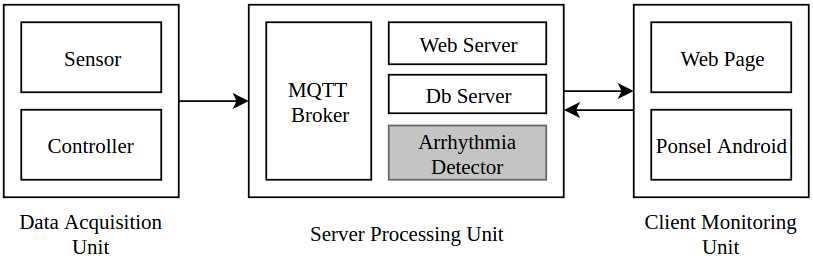
\includegraphics[scale=0.8]{images/gambar_umum.png}
    \caption{Gambaran Umum Sistem}
	\label{fig:gambar_umum}
\end{figure}

\section{Rancangan Perangkat Keras}
Sistem yang dirancang haruslah diimplementasikan untuk diuji coba. Oleh karena itu perlu dilakukan pemilihan perangkat keras. Perangkat keras dipilih berdasarkan pada kebutuhan rancangan sistem. Perangkat keras dibagi menjadi 3 bagian yaitu \textit{Receptor}, \textit{Server}, dan \textit{Viewer}.

Setelah perangkat keras ditentukan, algoritma yang sesuai untuk diterapkan harus dirancang. Rancangan algoritma terbagi menjadi 2 alur yaitu alur deteksi dan alur pemantauan. Rancangan algoritma dijelaskan lebih lengkap pada sub bab \ref{ssec:algorithm_design_1} dan sub bab \ref{ssec:algorithm_design_2}.

\subsection{Receptor}
Receptor berfungsi untuk mengambil data aktivitas jantung seorang pasien. Sistem yang dibangun tidak dapat menggunakan produk monitoring yang sudah ada karena sistem tersebut tidak bersifat \textit{Open Source}. Hal ini mengakibatkan penulis tidak bisa melakukan konfigurasi terhadap sensor dan \textit{controller}-nya. Konfigurasi yang dimaksud ialah menaikkan atau menurunkan frekuensi sampel dan transmit. Oleh karena itu penulis merancang receptor khusus untuk penelitian tugas akhir ini. Receptor dibangun dengan 3 komponen utama yaitu \textit{Sensor}, \textit{Controller}, dan baterai. Secara lengkap skema elektronik dapat dilihat pada gambar \ref{fig:schematics}.

\begin{figure}[H]
\centering
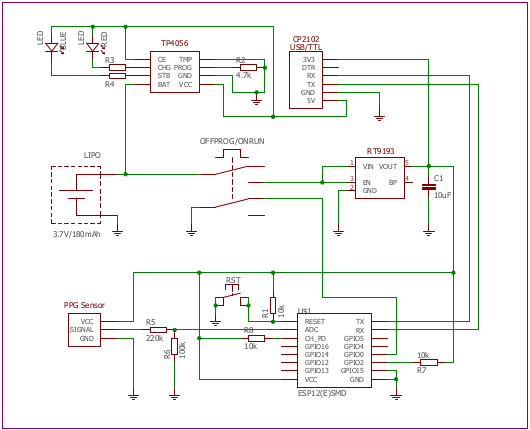
\includegraphics[scale=0.7]{images/schematics.png}
\caption{Skema Elektronik Receptor}
\label{fig:schematics}
\end{figure}

\subsubsection{Sensor}
Sistem dirancang untuk mengembangkan produk pemantauan jantung yang sudah ada di pasaran. Berdasarkan pengetahuan yang telah dibangun pada bab kajian pustaka, terdapat 2 jenis sensor yang umum digunakan yaitu ECG dan PPG. Berdasarkan rancangan algoritma pada sub bab \ref{ssec:algorithm_design} fitur yang dipilih dapat dihasilkan baik oleh ECG maupun PPG. Dengan demikian ECG dan PPG dapat digunakan dalam sistem.

Dalam tugas akhir ini, penulis memilih menggunakan PPG. Sensor PPG yang digunakan merupakan produksi Pulse Sensor yang dirancang oleh Joel dan Yury \cite{pulse_sensor}, terlihat pada gambar \ref{fig:coin_esp_pulse}. Alasan penulis milihan PPG ialah karena:
\begin{enumerate}
	\item harganya yang murah,
	\item PPG hanya menempel di satu bagian tubuh,
	\item PPG berukuran relatif kecil,
	\item kekurangan PPG yaitu kurang akurat dibanding ECG, tidak menyalahi tujuan sistem sebagai peringatan dini bukan medis.
\end{enumerate}

\subsubsection{Controller}
Sistem dirancang untuk monitoring terus menerus dan \textit{Ubiquitous}. Maka receptor haruslah cukup kecil untuk dibawa kemana saja dan menggunakan media komunikasi \textit{wireless} (tanpa kabel) untuk beriteraksi dengan server. Terdapat banyak jenis media komunikasi \textit{wireless} seperti GSM/CDMA, WiFi, Bluetooth, Infra Red, Zigbee, dll. WiFi dipilih sebagai media, pada sistem, karena jarak cakup yang cukup besar dan mudah untuk dikonfigurasi. Berdasarkan pengetahuan yang telah dibangun pada bab kajian pustaka, terdapat sebuah SoC yang telah memiliki kemampuan \textit{controller} dan memiliki modul WiFi dengan ukuran yang kecil yaitu ESP-12. Oleh karena itu receptor dirancang menggunakan ESP-12.

\subsubsection{Baterai}
Untuk memungkinkan receptor dibawa kemana saja dan dikenakan terus menerus diperlukan baterai sebagai catuan. Pada tugas akhir ini penulis menggunakan baterai \textit{Li-Polymer} (LiPo) \textit{protected} berkapasitas 180mAh dan tegangan 3.7V. Baterai ini juga berukuran kecil yaitu 25x18x8 mm dan memiliki bobot 5.3 gr, terlihat pada gambar \ref{fig:battery}.

\begin{figure}[H]
	\centering
	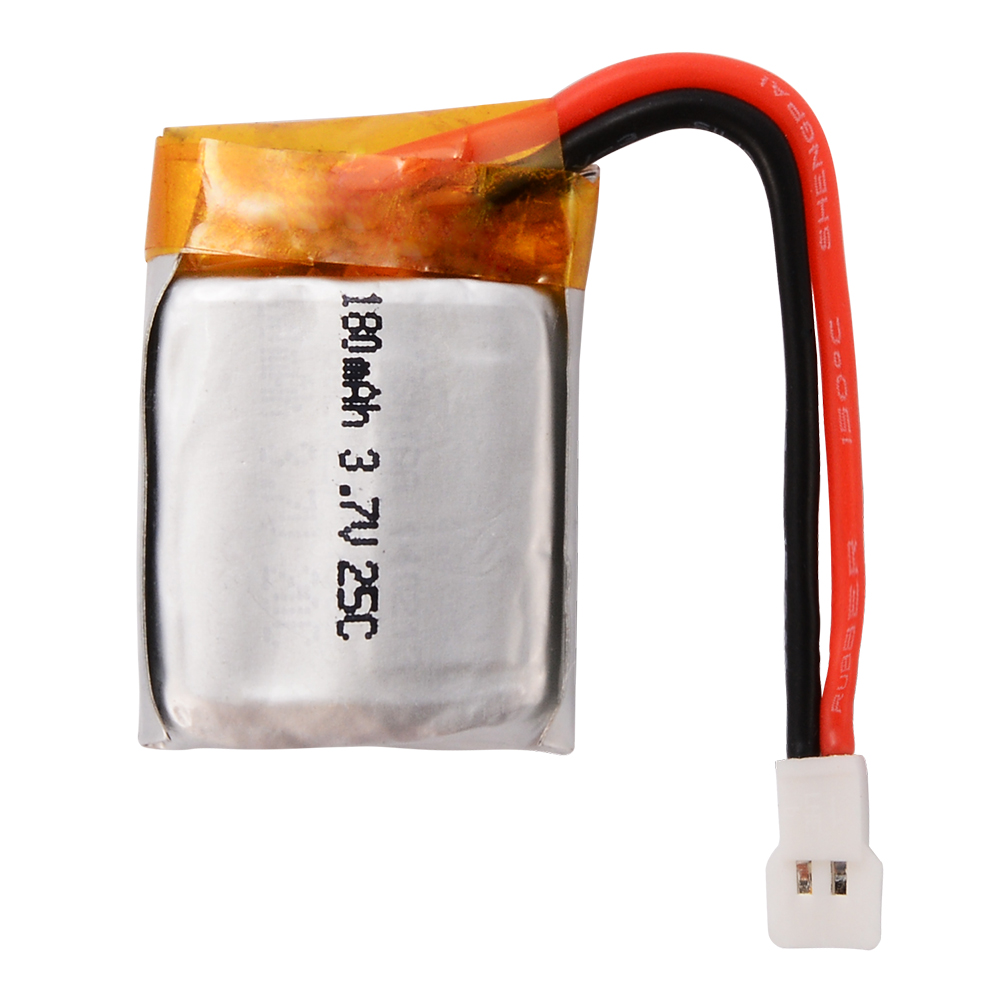
\includegraphics[scale=0.14]{images/baterai.jpg}
	\caption{Baterai LiPo 3.7v 180mAh}
	\label{fig:battery}
\end{figure}

\subsection{Server}
Untuk mengimplemantasikan konsep IoT server dirancang agar bisa melayani banyak \textit{receiver} dan \textit{viewer}. Oleh karena itu server harus melayani komunikasi dengan arus data yang tinggi. Alasan ini mendorong penulis memilih menggunakan protokol MQTT sebagai protokol komunikasi, NodeJs sebagai runtime dan MongoDb sebagai penyimpanan data. Server dirancang agar bisa berjalan pada satu perangkat. Hal ini berarti MQTT broker, Web server, DB server, dan Algoritma Detector berjalan pada satu alamat IP yang sama. 

\subsection{Viewer}
Sistem dirancang memiliki 2 saluran pemantauan yaitu halaman \textit{web} dan aplikasi pada ponsel Android. Kedua saluran ini dapat melakukan pemantauan selama berada dalam jaringan yang sama dengan server. Penulis memilih Android karena memiliki jumlah pengguna terbesar didunia[xx] sehingga bisa diasumsikan sistem yang dirancang bisa digunakan oleh banyak orang.

\subsubsection{Halaman Web}
Halaman web dibangun menggunakan \textit{framework} Express.Js. Pada halaman web terjadinya aritmia ditandai dengan bunyi dan bertambahnya angka hitungan aritmia yang terdeteksi. Tampilan halaman web dapat dilihat pada gambar \ref{fig:viewer_apps}.

\subsubsection{Aplikasi Ponsel Android}
Aplikasi ponsel android dibangun untuk dapat berjalan pada ponsel android ber-OS (\textit{operating system}) minimal Jelly Bean (Android v4.1). Pada aplikasi ini terjadinya aritmia ditandai dengan bunyi atau berubahnya status deteksi dan kode warna ikon seru. Kode warna merah berarti terdeteksi aritmia berbahaya, kuning terdeteksi aritmia tidak berbahaya, dan hijau berarti kondisi normal. Tampilan aplikasi android dapat dilihat pada gambar \ref{fig:viewer_apps}.

\begin{figure}[H]
	\centering
	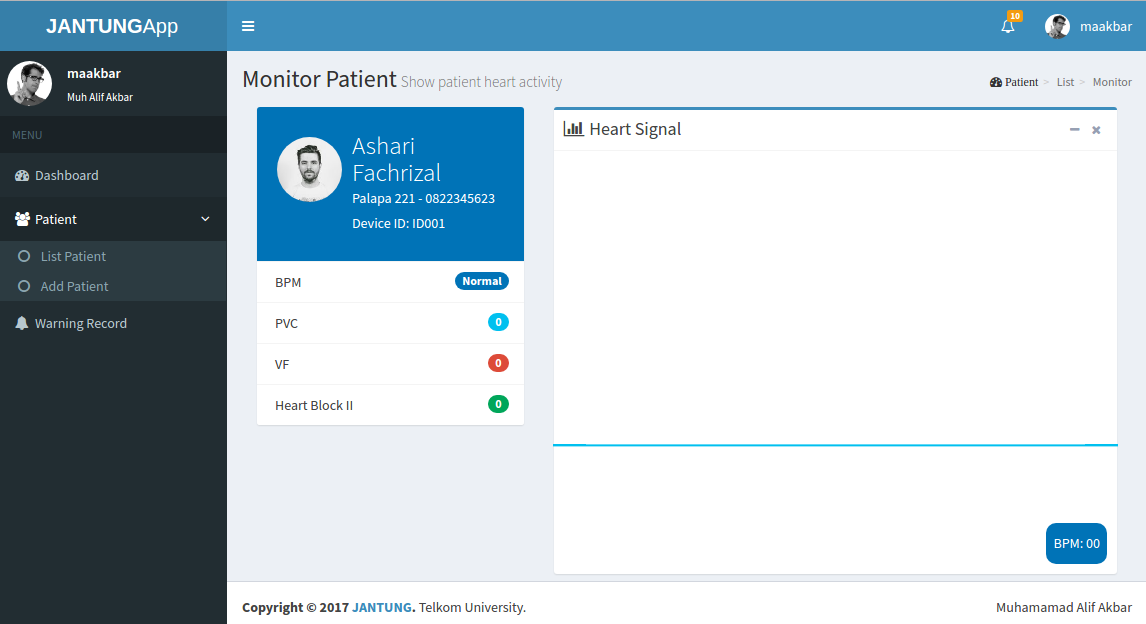
\includegraphics[scale=0.26]{images/web_app.png}
	\label{fig:viewer_apps}
	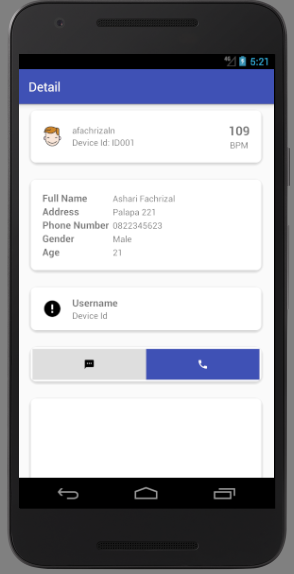
\includegraphics[scale=0.3]{images/phone_app.png}
	\caption{a) Tampilan Web Monitoring b) Tampilan Aplikasi Monitoring}
	\label{fig:viewer_apps}
\end{figure}

\section{Rancangan Algoritma Pemantauan} \label{ssec:algorithm_design_1}
Fungsi utama dari sistem yang dibuat ialah melakukan pemantauan. Untuk melakukan pemantauan sistem perlu mengaplikasikan algoritma pemantauan. Algoritma pemantauan hanya berjalan pada perangkat \textit{viewer} yaitu halaman \textit{web} atau aplikasi ponsel android. Alir algoritma pemantauan dapat dilihat pada gambar diagram alir \ref{flow:fig_report_algorithm}.
\begin{figure}[H]
	\centering
    %Mulai menggambar Flowchart
\begin{tikzpicture}[node distance=2cm]
\node (start) [cloud] {Start};
\node (open) [process, below of=start] {Membuka Viewer};
\node (input) [io, below of=open] {Memasukkan Kode Sensor / User};
\node (page) [process, below of=input] {Membuka Halaman Pemantauan};
\node (analysis) [process, below of=page] {Melakukan Analisis};
\node (stop) [cloud, below of=analysis] {Stop};
\draw [arrow] (start) -- (open);
\draw [arrow] (open) -- (input);
\draw [arrow] (input) -- (page);
\draw [arrow] (page) -- (analysis);
\draw [arrow] (analysis) -- (stop);
\end{tikzpicture}
    \caption{Flowchart Rancangan Algoritma Pemantauan}
	\label{flow:fig_report_algorithm}
\end{figure}

Seorang pengguna baik pasien, keluarga pasien, maupun dokter perlu membuka sebuah perangkat \textit{viewer}. Setelah aplikasi terbuka, baik web maupun aplikasi ponsel, user perlu memasukkan kode sensor atau user yang ingin dipantau. Setelah kode pantau dimasukkan aplikasi akan membuka halaman pemantauan. Setelah grafik pemantauan mulai berjalan pengguna bisa melakukan analisis.

\section{Rancangan Algoritma Deteksi} \label{ssec:algorithm_design_2}
Fungsi berikutnya yang akan diterapkan dalam sistem ialah dapat melakukan pendeteksian aritmia otomatis. Untuk itu sistem perlu menerapkan algoritma deteksi. Algoritma deteksi yang diterapkan pada tugas akhir ini terbagi menjadi 5 tahap yaitu Pengambilan dan Pengiriman Sinyal, Preprocessing dan Perekaman, Deteksi Detak Otomatis, Deteksi Aritmia Otomatis dan Pengiriman Laporan. Alir tahap algoritma deteksi digambarkan pada gambar diagram alir \ref{flow:fig_detect_algorithm}.

\begin{figure}[H]
	\centering
    %Mulai menggambar Flowchart
\begin{tikzpicture}[node distance=2cm]
\node (start) [cloud] {Start};
\node (get) [process, below of=start] {1. Pengambilan dan Pengiriman Sinyal};
\node (record) [process, below of=get] {2. Preprocessing dan Perekaman};
\node (beat) [process, below of=record] {3. Deteksi Detak Otomatis};
\node (aritmia) [process, below of=beat] {4. Deteksi Aritmia Otomatis};
\node (detected) [decision, below of=aritmia] {Terdeteksi?};
\node (report) [process, below of=detected] {5. Pengiriman Laporan};
\node (stop) [cloud, below of=report] {Stop};
\draw [arrow] (start) -- (get);
\draw [arrow] (get) -- (record);
\draw [arrow] (record) -- (beat);
\draw [arrow] (beat) -- (aritmia);
\draw [arrow] (aritmia) -- (detected);
\draw [arrow] (detected) -- (report);
\draw [arrow] (detected) -- ++(-80pt,0pt) |- (stop);
\draw [arrow] (report) -- (stop);
\end{tikzpicture}
    \caption{Flowchart Rancangan Algoritma Deteksi}
	\label{flow:fig_detect_algorithm}
\end{figure}

\subsection{Pengambilan dan Pengiriman Sinyal}
Pengambilan dan Pengiriman sinyal dilakukan di Receptor. Langkah pertama ialah \textit{controller} mengambil nilai pada pin analognya. Nilai pada pin analog lalu dikonversi menjadi satuan \textit{Volt}. Nilai yang telah dikonversi kemudian disisipkan header lalu dikirim  menggunakan protokol MQTT dengan QoS 0. \textit{Controller} kemudian tidur selama 2 ms lalu mengulang pengambilan dan pengiriman. Header berisi kode sensor dan angka index untuk menandakan urutan hasil bacaan. Index terebut direset setiap angka 1000. Diagram alir untuk memperjelas algoritma bagian ini dapat dilihat pada gambar \ref{flow:flow_sample}.

\begin{figure}[H]
\centering
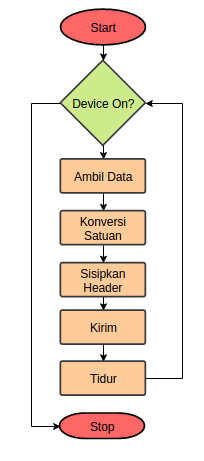
\includegraphics[scale=0.8]{images/flow_sample.png}
\caption{Flowchart Pengambilan dan Pengiriman Sinyal}
\label{flow:flow_sample}
\end{figure}

\subsection{Preprocessing dan Perekaman}
Setelah data diterima oleh server. Server melakukan \textit{preprocessing} pada data. \textit{Preprocessing} yang dilakukan terbagi menjadi \textit{data completer}, \textit{filtering}, \textit{squaring}, \textit{moving window integration}(MWI) dan \textit{Adaptive Thresholding}. Setelah \textit{filtering} dilakukan nilai dianggap telah bersih \textit{noise} maka nilai ini di simpan/rekam di \textit{database}. Preprocessing berlanjut ke \textit{squaring} dan MWI. Terakhir ekstraksi fitur \textit{peak} (R pada ECG dan Systolic pada PPG) dilakukan dengan \textit{Adaptive Thresholding}. Alir algoritma \textit{preprocessing} dapat dilihat pada diagram alir \ref{flow:fig_preproc_algorithm}. Rangkaian \textit{preprocessing} ini merupakan modifikasi pada algoritma yang diusulkan oleh Pan-Tomkin (1985) dan Kalidas-Tamil (2016) agar kedua algoritma ini bisa bekerja untuk ECG dan PPG.

\subsubsection{Data Completer}
Data Completion berfungsi ialah algoritma untuk menangani hilangnya data selama pengiriman. Hal ini mungkin terjadi karena data dikirimkan dari \textit{receptor} menggunakan QoS 0. Pertama, data dipisahkan antara nilai pembacaan sensor dan header. Header kemudian digunakan untuk memisahkan proses perhitungan, setiap kode sensor akan memiliki proses sendiri. Jika terdapat locatan index pada header (index data yg diterima bukan bertambah 1 dari index data sebelumnya) maka proses akan menambah data buffer sebanyak jumlah index yang terlompati dengan nilai berdasarkan proyeksi garis lurus dari nilai terakhir ke nilai terbaru mengikuti persamaan \ref{eq:line}. Jika tidak ada nilai yang hilang maka nilai akan langsung dimasukkan ke buffer.

\begin{equation}
y(n) = \dfrac{n (v_{2} - v_{1})}{d} + v_{1}
\label{eq:line}
\end{equation}

$v_{1}$ adalah nilai terakhir yang diterima, $v_{2}$ adalah nilai terbaru yang diterima, $n$ adalah jarak dari index terakhir, $d$ adalah jarak index terbaru ke terakhir. $y$ adalah nilai index $n$ yang hilang

\subsubsection{Filtering}
Filtering berfungsi untuk menghilangkan noise yang mempengaruhi sinyal. \textit{Noise} yang umum terdapat ialah \textit{muscle noise} dan \textit{baseline wander}. Filtering yang diterapkan terbagi menjadi dua tahap yaitu \textit{Band Pass Finite Impulse Response(FIR) Filter} kemudian \textit{First Order Derivation Filter}. Tahap ini sesuai dangan algoritma yang diusulkan oleh Pan-Tomkins (1985)\cite{pantom} dan Kalidas-Tamil (2016) \cite{ecg_syncro}. \textit{Band Pass Filter} yang digunakan memiliki frekuensi response 5-15Hz. Daftar koefisien lengkap untuk \textit{Band Pass Filter} dan \textit{Derivation Filter} tercantum pada tabel x.x di bab lampiran.

\subsubsection{Squaring dan MWI}
Sesuai namanya \textit{Squaring} melakukan penguadratan (persamaan \ref{eq:square}) terhadap data. Sedangkan MWI melakukan penghalusan data berdasarkan n data sebelum. MWI dilakukan dengan persamaan \ref{eq:mwi}.

\begin{equation}
y = x^{2}
\label{eq:square}
\end{equation}
\begin{equation}
y(n) = 2v_{n} + v_{n-1} - v_{n-3} - 2v_{n-4}
\label{eq:mwi}
\end{equation}

\begin{figure}[H]
	\centering
    %Mulai menggambar Flowchart
\begin{tikzpicture}[node distance=2cm]
\node (start) [cloud] {Start};
\node (get) [io, below of=start] {Input Data Jantung};
\node (band) [process, below of=get] {Band Pass Filter};
\node (derr) [process, below of=band] {Derivation Filter};
\node (save) [process, below of=derr] {Simpan Hasil};
\node (square) [process, below of=save] {Squaring};
\node (mwi) [process, below of=square] {MWI};
\node (stop) [cloud, below of=mwi] {Stop};
\draw [arrow] (start) -- (get);
\draw [arrow] (get) -- (band);
\draw [arrow] (band) -- (derr);
\draw [arrow] (derr) -- (save);
\draw [arrow] (save) -- (square);
\draw [arrow] (square) -- (mwi);
\draw [arrow] (mwi) -- (stop);
\end{tikzpicture}
    \caption{Flowchart Rancangan Algoritma Preprocessing}
	\label{flow:fig_preproc_algorithm}
\end{figure}

\subsection{Deteksi Detak Otomatis}
Hal penting untuk dideteksi pada aktivitas jantung ialah detaknya. Tanpa mendeteksi detak deteksi lainnya tidak dapat dilakukan. Deteksi detak dapat dilakukan dengan mencari titik \textit{fiducial}. Titik \textit{fiducial} yang paling menonjol ialah puncak tertinggi dari siklus detak yaitu R (pada ECG) dan Systolic (pada PPG). Untuk mendeteksi puncak dapat dilakukan dengan \textit{Adaptive Thresholding}. Algorima yang diterapkan merupakan modifikasi dari yang diusulkan Pan-Tompkins(1985). Pan-Tompkins(1985) mengusulkan teknik \textit{adaptive} dengan merubah nilai \textit{threshold} berdasarkan nilai puncak pada satu detak. Modifikasi yang diterapkan merubah \textit{threshold} berdasarkan rata-rata nilai pengukuran pada suatu durasi window. Peak ditentukan dengan cara mengambil nilai maksimum dari suatu wilayah yang melewati threshold (persamaan \ref{eq:threshold} dan \ref{eq:r_threshold}). Algoritma deteksi puncak dan penghilang puncak palsu dapat dilihat pada kolom algoritma \ref{Algo:peaksFind} dan \ref{Algo:peaksRemove}.

\begin{equation}
threshold = \alpha (\sum_{n=1}^{d} \frac{v_{n}}{d})
\label{eq:threshold} 
\end{equation}
\begin{equation}
rThreshold = \beta (\sum_{i=1}^{j} \frac{r_{i}}{j})
\label{eq:r_threshold} 
\end{equation}

Ket:
$\alpha$ merupakan variabel konstan untuk menaikkan threshold. $n$ menunjukan posisi sampel. $d$ merupakan durasi window, $n$ hingga jumlah sampel pada durasi tersebut. $v_{n}$ merupakan nilai bacaan pada sample ke-$n$.

$\beta$ merupakan variabel konstan untuk menaikkan threshold jarak RR. $i$ menunjukan index peak. $j$ total peak pada window. $r_{n}$ merupakan nilai jarak RR ke-$n$.

\begin{algorithm}[H]
 \begin{algorithmic}[1]
    \Function{peakFinder}{$window, \alpha, d$}
   	\State \text{threshold := $\alpha$ * mean($window, d$)}
	\ForAll{$sample \in window$} 
   	   	\If {$sample > threshold$}
	   		\If {$isPeakArea \neq true$}
	   			\State \text{isPeakArea := true}
				\State \text{tempPeak := sample}
				\State \text{peakCounter += 1}
				\State \text{peaksArea[peakCounter] := tempPeak}
			\ElsIf {$sample > tempPeak$}
				\State \text{tempPeak := sample}
				\State \text{peaksArea[peakCounter] := tempPeak}	
			\EndIf
	   	\Else
	   		\State \text{isPeakArea := false}
   		\EndIf
	\EndFor	
	\State \Return peaksArea
	\EndFunction
 \end{algorithmic}
 \caption{Fungsi Penentuan Peak}\label{Algo:peaksFind}
\end{algorithm} 

\begin{algorithm}[H]
 \begin{algorithmic}[1]
    \Function{falsePeakRemoval}{$peaksArea$}
	\State \text{rThreshold := $\beta$ * mean(distance($peaksArea$))}
	\ForAll{$peak_i \in peaksArea$} 
   	   	\If {$distance(peak_i, peak_{i-1}) < rThreshold$} \Comment{Calculate distance from $peak_i$ to $peak_{i-1}$}
	   		\State $remove(peak, peaksArea)$ \Comment{Remove peak from peak area}
   		\EndIf
	\EndFor	
	\State \Return peaksArea
	\EndFunction
 \end{algorithmic}
 \caption{Prosedur Filter False Peak}\label{Algo:peaksRemove}
\end{algorithm}

\subsection{Deteksi Aritmia Otomatis}
Deteksi Aritmia merupakan salah satu tujuan dari tugas akhir ini. Untuk melakukan deteksi aritmia pada tugas akhir ini menerapkan algoritma usulan Tsipouras(2005)\cite{rr_classification}. Algoritma ini dipilih karena kelebihannya yaitu dapat melakukan deteksi hanya menggunakan jarak antar titik R pada data ECG. Karena hanya menggunakan titik R, maka algoritma ini juga dapat secara langsung diterapkan pada data PPG. Pada penelitian Tsipouras (2005), ia membangun \textit{rule-based detector} berdasarkan masukan tim dokter jantung yang terlibat. \textit{Rule} ini dengan menggunakan sebuah (i) \textit{window RR-interval}, yang berisi 3 RR-interval, $RR1_i, RR2_i, RR3_i$.

Algoritma ini hanya dapat mendeteksi 4 kelompok aritimia. Pengelompokan aritmia ini dapat diihat pada tabel \ref{table:beat_class}. \textit{Rule} untuk pengelompokan ini dapat dilihat pada gambar \ref{Algo:rule}.

\begin{table}[H]
\centering
	\begin{tabular}{|L{2cm} | l | L{2cm}|}
	\hline
	\rowcolor{gray}
	\textbf{MIT-BIH Beat Symbol} & \textbf{Arti Symbol} & 	\textbf{Kategori} \\
	\hline
	N & Normal & 1 \\
	. & Normal &  \\
	/ & Paced Beat & \\ 
	f & Fusion of paced and normal beat & \\
	x & Non-conducted P-wave (blocked APB) & \\
	L & Left bundle branch block & \\ 
	R & Right bundle branch block & \\ 
	Q & Unclassifed & \\
	\hline
	V & PVC & 2 \\
	A & PAC & \\
	\hline
	! & VF & 3 \\
	\hline
	(BII & Heart block & 4 \\
	\hline
	\end{tabular}
	\caption{Pengelompokan Tipe beat}
	\label{table:beat_class}
\end{table}

\begin{figure}[H]
	\centering
	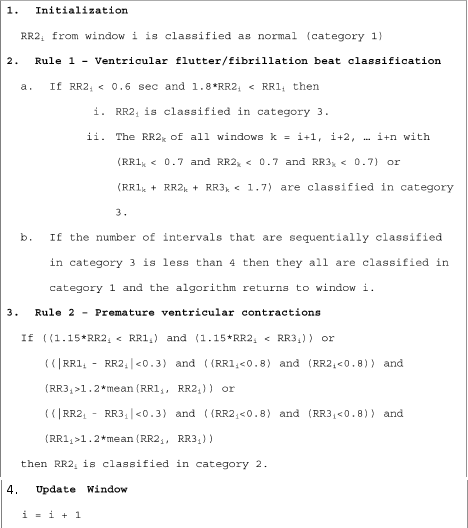
\includegraphics[scale=0.8]{images/algo_detect.png}
	\caption{\textit{Rule}/Algoritma yang diajukan Tsipouras (2005)}
	\label{Algo:rule}
\end{figure}

\subsection{Pengiriman Laporan}
Pengguna dapat menerima laporan atau melakukan pemantauan pada \textit{Viewer} mereka. Namun untuk menjaga perangkat \textit{Viewer} dapat me-\textit{render} tampilan dengan baik perlu dilakukan penurunan kecepatan sample (lihat diagram alir ). Selain itu \textit{Viewer} harus terus menerus terkoneksi dengan \textit{Server} untuk bisa mendapatkan data \textit{real-time}. Sehingga kapanpun \textit{server} mendeteksi aritmia pengguna dapat melihat peringatan pada device mereka. 

\begin{figure}[H]
\centering
    %Mulai menggambar Flowchart
\begin{tikzpicture}[node distance=2cm]
\node (start) [cloud] {Start};
\node (get) [io, below of=start] {Input Target FPS};
\node (getFrek) [io, below of=get] {Input Frekuensi Sampel};
\node (counter) [process, below of=getFrek] {counter:= Frek/FPS};
\node (drop) [process, below of=counter] {isDrop:= index mod counter != 0};
\node (dec) [decision, below of=drop] {isDrop?};
\node (send) [process, below of=dec] {Kirim \textit{filtered sample}};
\node (stop) [cloud, below of=send] {Stop};
\draw [arrow] (start) -- (get);
\draw [arrow] (get) -- (getFrek);
\draw [arrow] (getFrek) -- (counter);
\draw [arrow] (counter) -- (drop);
\draw [arrow] (drop) -- (dec);
\draw [arrow] (dec) -- (send);
\draw [arrow] (send) -- (stop);
\draw [arrow] (dec) -- ++(-90pt,0pt) |- (stop);
\end{tikzpicture}
    \caption{Flowchart Rancangan Algoritma Preprocessing}
	\label{flow:fig_preproc_algorithm}
\end{figure}

\subsection{Hubungan Algoritma Deteksi Dengan Perangkat Keras}
Hubungan antara algoritma deteksi dengan perangkat keras digambarkan pada gambar diagram tahap \ref{seq:fig_detect_algorithm2}. Seorang pasien yang mengenakan \textit{receptor} akan diambil data jantungnya kemudian dikirim ke \textit{server}. Ketika terdeteksi aritmia, \textit{server} akan mengirim \textit{flag} manandakan aritmia terdeteksi ke \textit{viewer} yang kemudian dilihat oleh pasien, dokter dan keluarga pasien.
\begin{figure}[H]
	\centering
	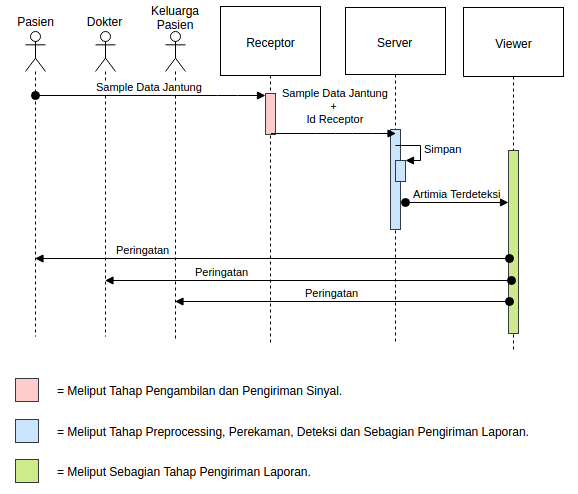
\includegraphics[scale=0.7]{images/sequence1.png}
	\caption{Diagram Tahap (\textit{Sequence}) Algoritma Deteksi}
	\label{seq:fig_detect_algorithm2}
\end{figure}

\section{Skenario Pengujian}
Untuk mengetahui keberahasilan seluruh rancangan diperlukan adanya pengujian, baik secara perangkat maupun algoritma. Hal ini ditujukan mengetahui apakah tujuan tugas akhir ini tercapai.

\subsection{Parameter Pengujian}
Berikut hubungan antara parameter penguji dengan tujuan tugas akhir:

\begin{table}[H]
	\begin{tabular}{|l|L{3cm}|L{2cm}|L{6cm}|}
	\hline
	\rowcolor{gray}
	\textbf{No} & \textbf{Parameter} & \textbf{Tujuan yg Dicakup} & \textbf{Alasan}\\
	\hline
	1 & Eksistensi Fitur & 2, 4 & Mengetahui apakah fitur yang direncanakan bisa berjalan. \\
	\hline
	2 & Delay & 1, 3, 4 & Dengan mengukur \textit{delay} dapat diketahui berapa lama proses pengiriman sehingga dapat diketahui seberapa \textit{Real Time} sistem dapat berjalan. \\
	\hline
	3 & Execution Time & 1, 2, 3, 4 & Dengan mengukur execution time dapat diketahui seberapa banyak sensor yang dapat ditangani oleh spesifikasi server tertentu \\
	\hline
	4 & FPS & 2, 4 & Dengan mengukur FPS dapat diketahui maksimum FPS agar dapat dijalankan pada banyak \textit{viewer} \\
	\hline
	5 & Akurasi & 3 & Dengan mengukur akurasi dapat diketahui seberapa akurat algoritma deteksi yang diterapkan \\
	\hline
	\end{tabular}
\end{table}

\subsection{Konfigurasi Perangkat Keras}
Spesifikasi perangkat keras yang digunakan selama pengujian dapat dilihat pada tabel \ref{tabel:spesifikasi}. Pengujian dilakukan dengan menghubungkan sebuah \textit{receiver}, kepada sebuah \textit{server} dan dipantau oleh 2 \textit{viewer} (web dan ponsel). Hubungan jaringan perangkat keras digambarkan pada gambar \ref{fig:konfigurasi}.

\begin{table}[H]
	\centering
	\begin{tabular}{|l|L{3cm}|L{8cm}|}
	\hline
	\rowcolor{gray}
	\textbf{No} & \textbf{Perangkat} & \textbf{Spesifikasi} \\
	1 & Receptor &
	\begin{itemize}
		\item ESP-12F
		\item Sensor Pulse
		\item Modul USB TTL CP2102
		\item IC TP4056 LiPo charger
		\item IC LDO regulator RT9193
		\item Battery LiPo protected 180mAh
	\end{itemize} \\
	\hline
	2 & Server & 
	\begin{itemize}
		\item Laptop ASUS A43SD
		\item Intel i3-2350M CPU @ 2.30GHz
		\item RAM DDR3 8GB
	\end{itemize} \\
	\hline
	3 & Viewer Web & 
	\begin{itemize}
		\item Laptop Lenovo G40S
		\item AMD A8 5550M CPU @ 2.1GHz
		\item RAM DDR3 8GB
	\end{itemize} \\
	\hline
	4 & Viewer Android & 
	\begin{itemize}
		\item ZTE A711, Android Lollipop
		\item Snapdragon 615 CPU @ 1.7 GHz
		\item RAM 2GB
	\end{itemize} \\
	\hline
	5 & WiFi Routers & 
	\begin{itemize}
		\item Jetfi G2
		\item WiFi IEEE 802.11b/g/n
	\end{itemize} \\
	\hline
	\end{tabular}
	\caption{Tabel Spesifikasi Perangkat Keras}
	\label{tabel:spesifikasi}
\end{table}

\begin{figure}
	\centering
	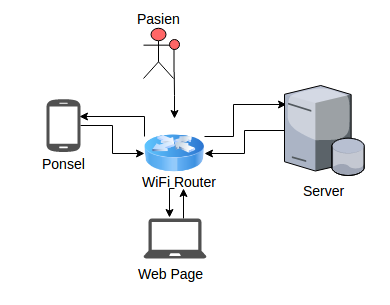
\includegraphics[scale=0.82]{images/konfigurasi.png}
	\caption{Konfigurasi Perangkat Keras}
	\label{fig:konfigurasi}
\end{figure}

\subsection{Pengujian Algoritma Pemantauan}
Sistem tidak bisa dites secara \textit{black box} (memberikan masukkan ke sistem dan melihat hasil) karena pengerjaan tugas akhir tidak didampingi oleh dokter ahli jantung untuk melakukan pengecekan atas hasil deteksi. Sehingga pengujian algoritma dipisah menjadi  2 tahap yaitu, algortima pemantauan dan algoritma deteksi. 

Pengujian algoritma pemantauan dilakukan dengan cara seseorang menggunakan \textit{receiver} dan dilihat keberhasilan pemantauan dari \textit{viewer}. Pengujian ini ditujukan untuk menguji semua parameter selain parameter 5 (Akurasi).

\subsubsection{Delay}
Delay yang diukur ialah waktu tempuh sejak dikirimnya data oleh \textit{receptor} hingga diterima oleh \textit{server}. \textit{Delay} dihitung dengan mengukur rata-rata selisih waktu ($t$) diterimanya data oleh server dikurang dengan waktu kerja sensor ($v$) (persamaan \ref{eq:delay}).

\begin{equation}
Delay = \alpha (\sum_{i=2}^{d} -\frac{(t_{i} - v_{i})}{d})
\label{eq:delay} 
\end{equation}

\subsubsection{Execution Time}
\textit{Execution Time} (Waktu eksekusi) diukur pada \textit{receptor} dan \textit{server}. Pada \textit{receptor} \textit{execution time} ialah waktu sejak sampel diambil hingga selesai dikirim ditambah waktu tidur antar sampel, waktu ini disebut sebagai waktu kerja sensor. Pada \textit{server} \textit{execution time} ialah waktu untuk memproses sebuah sampel hingga dimunculkannya sebuah deteksi. Karena pemrosesan dilakukan setiap sebuah \textit{window} terisi, maka \textit{execution time} yang dihitung dengan membagi durasi \textit{window} terhadap dengan jumlah sampel yang diproses (persamaan \ref{eq:exec_time}).

\begin{equation}
ET = (\frac{t_d}{d})
\label{eq:exec_time} 
\end{equation}

\subsubsection{FPS}
FPS diukur dengan mecoba konfigurasi \textit{downsample} pada \textit{server} dan melihat tampilan pada \textit{viewer}.

\subsection{Pengujian Algoritma Deteksi}
Pengujian algoritma deteksi dilakukan dengan memasukkan dataset ECG dari MIT-BIH Arrhythmia Database \cite{mit_bih_paper}\cite{mit_bih_web} ke dalam sistem. Untuk mempermudah visualisasi dan analisis data, penulis menjalankan algoritma deteksi pada bahasa pemograman python untuk selanjutnya diimplementasikan ke Node.Js. Pengujian ini ditujukan untuk menguji parameter akurasi.

\subsubsection{Dataset}
Dataset dari MIT-BIH \cite{mit_bih_paper}\cite{mit_bih_web} terbagi menjadi 48 \textit{records}. Masing masing \textit{record} memiliki panjang 30 menit. Dengan jumlah detak yang berbeda-beda. Rekapitulasi detak yang terekam pada dataset dapat dilihat pada tabel \ref{tabel:dataset}. Setiap \textit{record} telah dianotasi (ditandai) oleh dokter ahli jantung\cite{mit_bih_web}. Rekapitulasi anotasi pada dataset dapat dilihat pada tabel \ref{tabel:result1}  dan \ref{tabel:result2}.

\begin{table}[H]
	\centering
	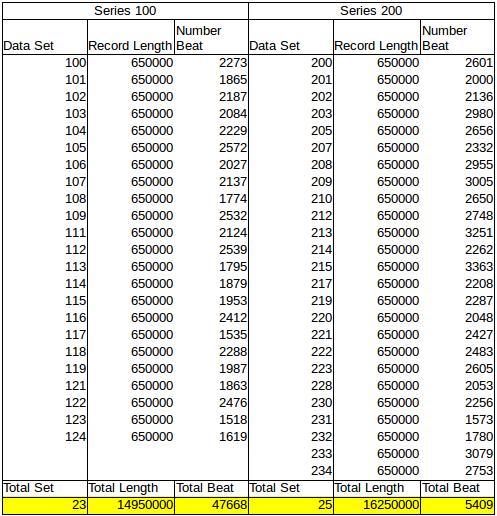
\includegraphics[scale=0.7]{images/tabel_data.png}
	\caption{Tabel Rakpitulasi Dataset}
	\label{tabel:dataset}
\end{table}	

\begin{table}[H]
	\centering
	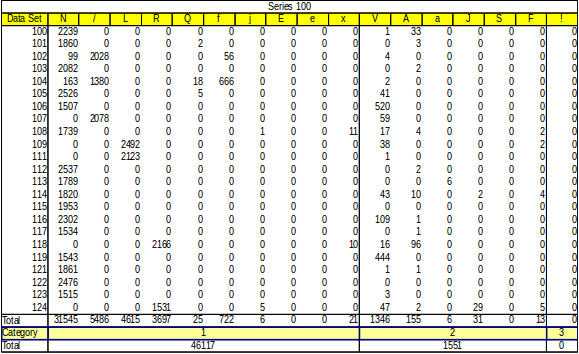
\includegraphics[scale=0.5]{images/result1.png}
	\caption{Tabel Rakpitulasi Aritmia series 100}
	\label{tabel:result1}
\end{table}
\begin{table}[H]
	\centering
	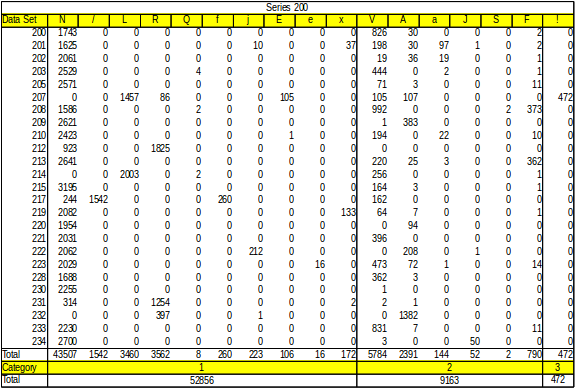
\includegraphics[scale=0.5]{images/result2.png}
	\caption{Tabel Rakpitulasi Aritmia series 200}
	\label{tabel:result2}
\end{table}

\subsubsection{Akurasi}
Pengukuran akurasi terbagi menjadi 2 yaitu akurasi deteksi detak dan akurasi deteksi aritmia. Untuk mengukur akurasi jumlah kelas (detak dan aritmia) digunakan persamaan \ref{eq:accuracy} dan \ref{eq:specificity}.

\begin{equation}
	Accuracy = \frac{TP + TN}{TP+TN+FP+FN}
	\label{eq:accuracy}
\end{equation}
\begin{equation}
	Specificity = \frac{TN}{TN+FP}
	\label{eq:precission}
\end{equation}

\begin{table}
	\centering
	\begin{tabular}{L{3cm}|C{3cm}|C{3cm}|}
	 & \textbf{Predicted: No} & \textbf{Predicted Yes} \\
	\hline
	\textbf{Actual: No} & TN & FP \\
	\hline
	\textbf{Actual: Yes} & FN & TP \\
	\hline	
	\end{tabular}
\end{table}


